\documentclass[documentclass]{jsarticle}
\usepackage[top=25truemm,bottom=25truemm,left=20truemm,right=20truemm]{geometry}
\usepackage{listings, jlisting, color}
\usepackage[dvipdfmx]{graphicx}
\usepackage{pdfpages}
\usepackage{amsmath}
\usepackage{amssymb, latexsym}
\usepackage{mathtools}
\usepackage{multirow}
\usepackage{color}
\usepackage{ulem}
\usepackage{here}
\usepackage{wrapfig}
\usepackage{tikz}
% 使用する関数の宣言
% (最低限これさえ宣言していれば十分だと思われるものを書いています)
\usetikzlibrary{intersections, calc, arrows, positioning, arrows.meta}


\newcommand{\Add}[1]{\textcolor{red}{#1}}
\newcommand{\Erase}[1]{\textcolor{red}{\sout{\textcolor{black}{#1}}}}
\newcommand{\ctext}[1]{\raise0.2ex\hbox{\textcircled{\scriptsize{#1}}}}

\lstset{
  basicstyle={\small},
  breaklines=true,
  frame=single,
  tabsize=3,
  numbers=left
}

\begin{document}
\title{情報理論 第8回 計算機演習}
\author{222C1021 今村優希}
\maketitle

\newpage

\section*{演習1}

\begin{figure}[H]
  \begin{center}
    \includegraphics*[scale=0.5]{figure/1-1.png}
  \end{center}
  \caption{2つの情報源の発生確率}
  \label{fig:1-1}
\end{figure}

上記の図\ref*{fig:1-1}の2つの情報源の値から相互情報量を求める.
まずは,それぞれの周辺確率を求める.
\begin{align*}
  P_X(0) &= \sum_j P_{X, Y}(0, y_j) = P_{X, Y}(0, 0) + P_{X, Y}(0, 1) = 0.55 + 0.05 = 0.60\\
  P_X(1) &= \sum_j P_{X, Y}(1, y_j) = P_{X, Y}(1, 0) + P_{X, Y}(1, 1) = 0.15 + 0.25 = 0.40\\
  P_Y(0) &= \sum_i P_{X, Y}(x_i, 0) = P_{X, Y}(0, 0) + P_{X, Y}(1, 0) = 0.55 + 0.15 = 0.70\\
  P_Y(1) &= \sum_i P_{X, Y}(x_i, 1) = P_{X, Y}(0, 1) + P_{X, Y}(1, 1) = 0.05 + 0.25 = 0.30  
\end{align*}
この確率から$X, Y$それぞれのエントロピーを求める.
\begin{align*}
  H(X) &= -0.6\log_2{0.6} - 0.4\log_2{0.4} = 0.442 + 0.529 = 0.971\\
  H(Y) &= -0.7\log_2{0.7} - 0.3\log_2{0.3} = 0.881
\end{align*}
さらに,周辺確率から条件確率$P_{X|Y}(x_i|y_j)=\dfrac{P_{X,Y}(x_i,y_j)}{P_Y(y_j)}$を求める.
\begin{align*}
  P_{X|Y}(0|0) &= \dfrac{P_{X,Y}(0,0)}{P_Y(0)}= \dfrac{0.55}{0.7} = 0.786\\
  P_{X|Y}(0|1) &= \dfrac{P_{X,Y}(0,1)}{P_Y(1)}= \dfrac{0.05}{0.3} = 0.167\\
  P_{X|Y}(1|0) &= \dfrac{P_{X,Y}(1,0)}{P_Y(0)}= \dfrac{0.15}{0.7} = 0.214\\
  P_{X|Y}(0|0) &= \dfrac{P_{X,Y}(1,1)}{P_Y(1)}= \dfrac{0.25}{0.3} = 0.833
\end{align*}
これを用いて条件付きエントロピーを求める.
先に,$H(X|Y=0)$と$H(X|Y=1)$を求める.
\begin{align*}
  H(X|Y=0) &= -P_{X|Y}(0|0) \log_2 P_{X|Y}(0|0) - P_{X|Y}(1|0) \log_2 P_{X|Y}(1|0)\\
  &= -0.786 \log_2 0.786 - 0.214 \log_2 0.214\\
  &= 0.749\\
  H(X|Y=1) &= -P_{X|Y}(0|1) \log_2 P_{X|Y}(0|1) - P_{X|Y}(1|1) \log_2 P_{X|Y}(1|1)\\
  &= -0.167 \log_2 0.167 - 0.833 \log_2 0.833\\
  &= 0.651
\end{align*}
\begin{align*}
  H(X|Y) &= \sum_j P_Y(y_i)H(X|Y=y_i)\\
  &= P_Y(0)H(X|Y=0) + P_Y(1)H(X|Y=1)\\
  &= 0.7 \cdot 0.749 + 0.3 \cdot 0.651
  &= 0.720
\end{align*}
以上の結果から,相互情報量$I(X;Y)$を求めると,
\begin{align*}
  I(X;Y) = H(X) - (X|Y) = 0.971 - 0.720 = 0.251
\end{align*}
したがって,相互情報量$I(X;Y)$は,$0.251$である.
\newpage

\section*{演習2}
\subsection*{演習2-1}
作成した状態遷移図は図\ref*{fig:2-1}である.
ラーメンを$S_1$,そばを$S_2$,うどんを$S_3$で作成を行った.
\begin{figure}[H]
  \begin{center}
    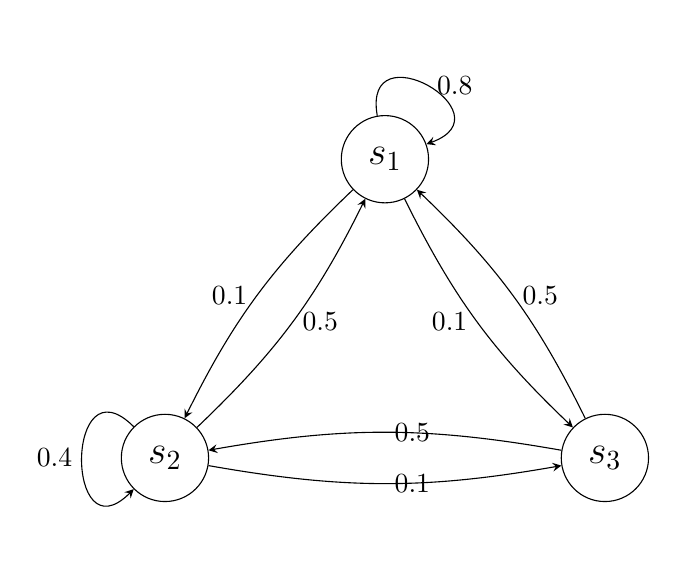
\begin{tikzpicture}[node/.style={draw, circle, font=\Large, inner sep=6pt}]
      \node[node] (s1) {$s_{1}$};
      \node[node, below left = 3cm and 2cm of s1] (s2) {$s_{2}$};
      \node[node, below right  = 3cm and 2cm of s1] (s3) {$s_{3}$};
  
      \path[->, >=stealth]
        (s1) edge[loop right, in=20, out=100, looseness=4] node{0.8} (s1)
        (s1) edge[left, bend right=10] node{0.1} (s2)
        (s1) edge[left, bend right=10] node{0.1} (s3)
        (s2) edge[right, bend right=10] node{0.5} (s1)
        (s2) edge[loop left, in=225, out=135, looseness=4] node{0.4} (s2)
        (s2) edge[right, bend right=10] node{0.1} (s3)
        (s3) edge[right, bend right=10] node{0.5} (s1)
        (s3) edge[right, bend right=10] node{0.5} (s2);
    \end{tikzpicture}
  \end{center}
  \caption{状態遷移図}
  \label{fig:2-1}
\end{figure}

\subsection*{演習2-2}
遷移確率行列を求めるために用いた$\prod$は,
\begin{align*}
  \prod = 
  \begin{pmatrix}
    0.8 & 0.1 & 0.1 \\
    0.5 & 0.4 & 0.1 \\
    0.5 & 0.5 & 0 
  \end{pmatrix}
\end{align*} 
である.$\prod^2, \prod^3, ... ,\prod^{10}, \prod^{50}, \prod^{100}$を算出するために以下のようなプログラムを作成し,matlabでの実行を行った.
5行目で初期の行列の入力を行い,7行目以下で行列の計算及び出力を行っている.

\begin{lstlisting}[caption=遷移確率行列を求めるプログラム]
  %情報理論
  %222C1021 今村優希
  %演習問題2-2 Πの2~10,50,100乗を求める問題
  
  A = [0.8 0.1 0.1; 0.5 0.4 0.1; 0.5 0.5 0]; %行列の入力
  
  %Π^1~Π^10までの計算と値の出力
  for c = 1:10
      x_1_10 = A^c;
      disp(c);
      disp(x_1_10);
  end
  
  %Π^50の計算と値の出力
  X_50 = A^50;
  disp(50);
  disp(X_50);
  %Π^100の計算の値と出力
  X_100 = A^100;
  disp(100);
  disp(X_100);
\end{lstlisting}

このプログラムを実行した結果がソースコード2である.
1行目の1が$\prod^1$を表しており,その結果が3から5行目に行列として出力されている.

\begin{lstlisting}[caption=遷移確率行列を求めるプログラム]
  1

  0.8000    0.1000    0.1000
  0.5000    0.4000    0.1000
  0.5000    0.5000         0

   2

  0.7400    0.1700    0.0900
  0.6500    0.2600    0.0900
  0.6500    0.2500    0.1000

   3

  0.7220    0.1870    0.0910
  0.6950    0.2140    0.0910
  0.6950    0.2150    0.0900

   4

  0.7166    0.1925    0.0909
  0.7085    0.2006    0.0909
  0.7085    0.2005    0.0910

   5

  0.7150    0.1941    0.0909
  0.7126    0.1965    0.0909
  0.7126    0.1966    0.0909

   6

  0.7145    0.1946    0.0909
  0.7138    0.1953    0.0909
  0.7138    0.1953    0.0909

   7

  0.7143    0.1947    0.0909
  0.7141    0.1950    0.0909
  0.7141    0.1950    0.0909

   8

  0.7143    0.1948    0.0909
  0.7142    0.1949    0.0909
  0.7142    0.1949    0.0909

   9

  0.7143    0.1948    0.0909
  0.7143    0.1948    0.0909
  0.7143    0.1948    0.0909

  10

  0.7143    0.1948    0.0909
  0.7143    0.1948    0.0909
  0.7143    0.1948    0.0909

  50

  0.7143    0.1948    0.0909
  0.7143    0.1948    0.0909
  0.7143    0.1948    0.0909

 100

  0.7143    0.1948    0.0909
  0.7143    0.1948    0.0909
  0.7143    0.1948    0.0909
\end{lstlisting}

\subsection*{演習2-3}
定常確率の計算を行う.
演習2-1にて作成した状態遷移図から以下の連立方程式が得られる.
\begin{equation}
  \left\{ \,
      \begin{aligned}
      & P(S_1) = 0.8P(S_1) + 0.5P(S_2) + 0.5P(S_3) \\
      & P(S_2) = 0.1P(S_1) + 0.4P(S_2) + 0.5P(S_3) \\
      & P(S_3) = 0.1P(S_1) + 0.1P(S_2) \label{sq:1}
      \end{aligned}
  \right.
\end{equation}
また,確率の総和は1なので,
\begin{align}
  P(S_1) + P(S_2) + P(S_3) = 1 \label{sq:2}
\end{align}
も成り立つ.数式(\ref*{sq:1})と(\ref*{sq:2})を用いて連立方程式を解くと,以下の結果が得られた.
\begin{equation*}
  \left\{ \,
    \begin{aligned}
      &P(S_1) = \dfrac{5}{7} = 0.714\\
      &P(S_2) = \dfrac{15}{77} = 0.195\\
      &P(S_3) = \dfrac{1}{11} = 0.091
    \end{aligned}
  \right.
\end{equation*}
この結果から,$\prod^{100}$の値における1列目が$P(S_1)$,2列目が$P(S_2)$,3列目が$P(S_3)$とほとんど同じ値を出力していることがわかった.
それぞれの列が定常確率を表していると思われる. 
このことから,$\prod$の乗数を大きくすれば,それぞれの列の値が定常確率に近づいていることが確認できる.


\subsection*{演習2-4}
演習2-3で求めた定常確率からエントロピーを計算する.
\begin{align*}
  H(X) &= -\dfrac{5}{7} \log_2 \dfrac{5}{7} -\dfrac{15}{77} \log_2 \dfrac{15}{77} - \dfrac{1}{11} \log_2 \dfrac{1}{11}\\ 
  &= 0.347 + 0.460 + 0.314\\
  &= 1.120
\end{align*}
と求めた.

\newpage

\section*{演習3}
\subsection*{演習3-1}
50回遷移するように設計したプログラムは,ソースコード3である.
11行目のStudentIDを021に設定した.
また,50回遷移するから,NIterationを「50」に,さらに62行目も「1:50」に変更した.
このプログラムをmatlabで実行した結果が,ソースコード4である.
また,遷移した状態の回数を棒グラフで表したものが図\ref*{fig:3-1}である.
\begin{lstlisting}[caption=状態変化を見るプログラム]
  % 九州工業大学情報工学部情報・通信工学科3年
% 情報理論 演習課題1 演習3
% 2024/05/10 黒崎正行
% 2024/05/10 今村優希一部変更

clear;                                 
clearvars -global;                    
close all;                            
clc;                                   
%% Parameter setting
StudentID = 021;            % 学籍番号の下3桁に変更すること
seed = StudentID;           % 学籍番号を乱数のシード値に設定
rng(seed);                  % 乱数のシード値の設定

CurrentState = 1;           % 現在の状態 (初期状態1)
NextState = 1;              % 次の状態 

NIteration = 50;          % 繰返し回数

StateHist = zeros(1, NIteration);

%% Start simulation
for ite = 1: NIteration

    Transition = rand;                                    % ランダム値の生成
    StateHist(ite) = CurrentState;                        % 現在の状態の番号を格納

    switch CurrentState
        case 1                                            % 状態1における動作を記述
            if Transition < 0.8                           % 0.8の確率で状態1に遷移
                NextState = 1;
            elseif Transition >= 0.8 && Transition < 0.9  % 0.9-0.8=0.1の確率で状態2に遷移
                NextState = 2;
            else                                          % 0.1の確率で状態3に遷移
                NextState = 3;
            end
        case 2                                            % 状態2における動作を記述
            if Transition < 0.5                           % 0.5の確率で状態1に遷移
                NextState = 1;
            elseif Transition >= 0.5 && Transition < 0.9  % 0.9-0.5=0.4確率で状態2に遷移
                NextState = 2;
            else                                          % 0.1の確率で状態2に遷移
                NextState = 3;
            end
        case 3                                            % 状態3における動作を記述
            if Transition < 0.5                           % 0.3の確率で状態1に遷移
                NextState = 1;
            elseif Transition >= 0.5 && Transition < 1.0  % 1.0-0.5=0.5の確率で状態2に遷移
                NextState = 2;
            else                                          % 0の確率で状態2に遷移
                NextState = 3;
            end
        otherwise
            NextState=1;
    end
    CurrentState = NextState;
end

%% Evaluation
% 最初から50回の遷移を表示
disp('State History');
disp(StateHist(1:50));

% ヒストグラムのグラフの表示
h = histogram(StateHist);

% 頻度の表示
%
 disp('State Frequency');
 disp('State   Count   Percent');
 fprintf('   S1, %6d, %8.3f %%\n', h.Values(1),h.Values(1)/NIteration*100);
 fprintf('   S2, %6d, %8.3f %%\n', h.Values(2),h.Values(2)/NIteration*100);
 fprintf('   S3, %6d, %8.3f %%\n', h.Values(3),h.Values(3)/NIteration*100);

\end{lstlisting}

\begin{lstlisting}[caption=ソースコード3を実行したときの結果]
  State History
  1 列から 20 列

     1     1     1     1     1     1     1     1     1     1     1     1     2     1     1     1     2     2     3     2

  21 列から 40 列

     1     1     1     1     2     3     2     2     1     1     1     1     1     1     1     1     1     2     1     1

  41 列から 50 列

     1     1     1     2     2     2     1     2     2     2

State Frequency
State   Count   Percent
   S1,     34,   68.000 %
   S2,     14,   28.000 %
   S3,      2,    4.000 %
\end{lstlisting}

\begin{figure}[H]
  \begin{center}
    \includegraphics*[scale=0.6]{figure/3-1.png}
  \end{center}
  \caption{50回遷移させたときの各状態に遷移した回数}
  \label{fig:3-1}
\end{figure}

\subsection*{演習3-2}
利用したプログラムは演習3-1で使用したソースコード3を一部変更したものである.
1000回遷移するから,NIterationを「1000」に,さらに62行目も「1:1000」に変更した.
出力はソースコード5で表しており,遷移した状態の回数を棒グラフで表したものが図\ref*{fig:3-2}である.
\begin{lstlisting}[caption=1000回遷移させるためのプログラム]
  % 九州工業大学情報工学部情報・通信工学科3年
% 情報理論 演習課題1 演習3
% 2024/05/10 黒崎正行
% 2024/05/10 今村優希改変

clear;                                 
clearvars -global;                    
close all;                            
clc;                                   
%% Parameter setting
StudentID = 021;            % 学籍番号の下3桁に変更すること
seed = StudentID;           % 学籍番号を乱数のシード値に設定
rng(seed);                  % 乱数のシード値の設定

CurrentState = 1;           % 現在の状態 (初期状態1)
NextState = 1;              % 次の状態 

NIteration = 1000;          % 繰返し回数

StateHist = zeros(1, NIteration);

%% Start simulation
for ite = 1: NIteration

    Transition = rand;                                      % ランダム値の生成
    StateHist(ite) = CurrentState;                          % 現在の状態の番号を格納

    switch CurrentState
        case 1                                              % 状態1における動作を記述
            if Transition < 0.8                             % 0.8の確率で状態1に遷移
                NextState = 1;
            elseif Transition >= 0.8 && Transition < 0.9    % 0.9-0.8=0.1の確率で状態2に遷移
                NextState = 2;
            else                                            % 0.1の確率で状態3に遷移
                NextState = 3;
            end
        case 2                                              % 状態2における動作を記述
            if Transition < 0.5                             % 0.5の確率で状態1に遷移
                NextState = 1;
            elseif Transition >= 0.5 && Transition < 0.9    % 0.9-0.5=0.4確率で状態2に遷移
                NextState = 2;
            else                                            % 0.1の確率で状態2に遷移
                NextState = 3;
            end
        case 3                                              % 状態3における動作を記述
            if Transition < 0.5                             % 0.3の確率で状態1に遷移
                NextState = 1;
            elseif Transition >= 0.5 && Transition < 1.0    % 1.0-0.5=0.5の確率で状態2に遷移
                NextState = 2;
            else                                            % 0の確率で状態2に遷移
                NextState = 3;
            end
        otherwise
            NextState=1;
    end
    CurrentState = NextState;
end

%% Evaluation
% 最初から1000回の遷移を表示
disp('State History');
disp(StateHist(1:1000));

% ヒストグラムのグラフの表示
h = histogram(StateHist);

% 頻度の表示
%
 disp('State Frequency');
 disp('State   Count   Percent');
 fprintf('   S1, %6d, %8.3f %%\n', h.Values(1),h.Values(1)/NIteration*100);
 fprintf('   S2, %6d, %8.3f %%\n', h.Values(2),h.Values(2)/NIteration*100);
 fprintf('   S3, %6d, %8.3f %%\n', h.Values(3),h.Values(3)/NIteration*100);

\end{lstlisting}

\begin{lstlisting}[caption=ソースコード5を実行した際の結果]
  State History
  1 列から 20 列

     1     1     1     1     1     1     1     1     1     1     1     1     2     1     1     1     2     2     3     2

  21 列から 40 列

     1     1     1     1     2     3     2     2     1     1     1     1     1     1     1     1     1     2     1     1

  % 一部省略 %

  941 列から 960 列

     1     2     2     1     1     1     1     2     2     2     1     3     2     1     1     2     2     2     1     1

  961 列から 980 列

     1     3     2     1     1     2     2     1     1     2     2     1     3     2     2     2     2     1     1     2

  981 列から 1,000 列

     2     1     2     2     1     1     1     1     1     1     3     1     1     1     1     1     1     1     2     2

State Frequency
State   Count   Percent
   S1,    713,   71.300 %
   S2,    195,   19.500 %
   S3,     92,    9.200 %
\end{lstlisting}

\begin{figure}[H]
  \begin{center}
    \includegraphics*[scale=0.6]{figure/3-2.png}
  \end{center}
  \caption{1000回遷移させたときの各状態に遷移した回数}
  \label{fig:3-2}
\end{figure}

\subsection*{演習3-3}
演習3-2の遷移する回数と初期状態を変更した以下の条件で実行した際の各確率に関して調べた.
\paragraph*{初期状態$S_2$で50回遷移させたとき}
\begin{align*}
 P(S_1) &= 66.0\%\\
 P(S_2) &= 30.0\%\\
 P(S_3) &= 4.0\%
\end{align*}
\paragraph*{初期状態$S_2$で1000回遷移させたとき}
\begin{align*}
  P(S_1) &= 71.2\%\\
  P(S_2) &= 19.6\%\\
  P(S_3) &= 9.2\%
 \end{align*}
\paragraph*{初期状態$S_3$で50回遷移させたとき}
\begin{align*}
  P(S_1) &= 66.0\%\\
  P(S_2) &= 28.0\%\\
  P(S_3) &= 6.0\%
 \end{align*}
\paragraph*{初期状態$S_3$で1000回遷移させたとき}
\begin{align*}
  P(S_1) &= 71.2\%\\
  P(S_2) &= 19.5\%\\
  P(S_3) &= 9.3\%
\end{align*}

\subsection*{演習3-4}
演習2と演習3の結果を見比べてみると,状態遷移を1000回遷移させたときの$S_1$から$S_3$それぞれに遷移する確率が演習2で求めた定常確率とほぼ同じである事がわかる.
したがって,定常確率$P(S_1)$はある時間において,状態$S_1$の確率も表しているとも言えると考える.

また,初期状態を変更したとしても各状態の発生確率はさほど変わらなかったことから,初期状態は発生確率に関係ないことがわかる.

\newpage

\section*{演習4}
\subsection*{演習4-1}
ZIPのアルゴリズムに関して説明する.データ圧縮は一般に「2段ロケット方式」が用いられている.
「2段ロケット方式」とはその名の通り,1段目の圧縮と2段目の圧縮が存在し,その2つをうまく組み合わせることで効率的な圧縮を実現している.

ZIPに関しては,1段目に「スライド辞書」方式を使用している.
辞書と呼ばれるエリアを確保して,その中から事前に出現した文字を探し出し,「その文字列と同じであること」を出力することで文字列を圧縮することができる.
1段目で文字列を圧縮できたので,2段目には「ハフマン符号」を用いてビット列にする.
ハフマン符号とは,可変長のビットを割り当てるアルゴリズムである.
出現頻度が多ければ多いほど短い符号に割り当て,その逆の場合は比較的長い符号が割り当てられる.
この事によって,文字列をビットに変換し圧縮することが可能である.

ただ,上記のハフマン符号の処理を実現するためには複数の支援機能が必要である.
まずは,符号として処理するためにビット単位に変換するための「ビットストリーム」,
単位にデータを溜め込んで頻度表を作る「バッファブロック」,
そのバッファブロク単位にビット長テーブル(頻度表)を入出力する処理も必要である.

ZIP圧縮の流れとしては,まずはスライド辞書に読み込まれ,一致文字列と不一致文字列の大きく2種類のコードに分解され,バッファにブロックに溜め込まれる.
その後,一定量溜め込まれたコードはハフマン符号期によってビットパターンに変換される.
そのビットパターンは可変長なので,ビットストリームを使ってバイト単位に出力することで圧縮が完了する.
これらの流れを図示したものが図\ref*{fig:4-1}である.
\begin{figure}[H]
  \begin{center}
    \includegraphics*[scale=0.5]{figure/4-1.png}
  \end{center}
  \caption{ZIP圧縮アルゴリズムのモデル}
  \label{fig:4-1}
\end{figure}

\subsection*{演習4-2}
用意したファイルとその容量は以下の表\ref*{tb:4-1}の通りである.
テキストファイルの文字コードはUTF-8である.
\begin{table}[H]
  \begin{center}
    \caption{用意したファイルとその容量}
    \label{tb:4-1}
    \begin{tabular}{|cc|} \hline
     ファイルの種類 & ファイルの容量 \\ \hline
     .txt    & 3,204,504バイト \\
     .jpeg   & 149,984 バイト \\
     .mp3    & 74,196,385 バイト \\ \hline
    \end{tabular}
  \end{center}
\end{table}

\subsection*{演習4-3}
zip圧縮はwindows標準搭載のものを使用した.
圧縮後の容量をまとめたものが表\ref*{tb:4-2}である.
\begin{table}[h]
  \begin{center}
    \caption{用意したファイルとその容量}
    \label{tb:4-2}
    \begin{tabular}{|cc|} \hline
     ファイルの種類 & 圧縮ファイルの容量 \\ \hline
     .txt    & 3,240 バイト \\
     .jpeg   & 137,581  バイト \\
     .mp3    & 73,670,682  バイト \\ \hline
    \end{tabular}
  \end{center}
\end{table}

\subsection*{演習4-4}
圧縮率の比較を行う.比較した結果を表\ref*{tb:4-3}にまとめた.
圧縮率は
\begin{align*}
  圧縮率 = \dfrac{圧縮前のファイル容量}{圧縮後のファイル容量}
\end{align*}
で計算を行った.
\begin{table}[h]
  \begin{center}
    \caption{それぞれのファイルの圧縮率}
    \label{tb:4-3}
    \begin{tabular}{|cc|} \hline
     ファイルの種類 & 圧縮率 \\ \hline
     .txt    &  $1.011 \times 10^{-3}$\\
     .jpeg   & $0.917$ \\
     .mp3    & $0.993$ \\ \hline
    \end{tabular}
  \end{center}
\end{table}

\subsection*{演習4-5}
演習4-2から4をもとに,それぞれのファイル圧縮率に関して考察を行う.
演習4-1のZIP圧縮のアルゴリズムから,ZIP圧縮は文字列に対して非常に有効であると考えられる.
したがって,テキストファイルの圧縮率が非常に小さいことから,効率的に圧縮が行われていることが伺える.
一方,文字列に対してjpgやmp3の圧縮率は非常に大きく,効率的に圧縮が行われてないと思われる.
jpegもmp3もすでに圧縮されたファイルであり,文字列ではないのでZIPでの圧縮が効率的に行われなかったと考えられる.

追記(一回消えたのでバックアップからの出力で一部間違いがあるかも)

\newpage
\begin{thebibliography}{9}
  \bibitem{1} 奥村晴彦 山崎敏,LHAとZIP : 圧縮アルゴリズム×プログラミング入門, ソフトバンク パブリッシング株式会社, 東京, 2003.
  \bibitem{2} SHARP, デジタルカメラで撮影した画像をZIP形式に圧縮してもファイルサイズが小さくならない Q&A情報(文書番号:107790)\\
  https://cs.sharp.co.jp/faq/qa?qid=107790, 参照:20245/19.
\end{thebibliography}
\end{document}